\section{Single View Geometry}
\begin{wrapfigure}{r}{4cm}
	
\includegraphics[scale=0.35]{figures/pic_1.png}
	\caption{一张风景图}
\end{wrapfigure}
上面我们解释了从3D转换到2D的过程,那么反过来,能否从单视角还原成3D呢?很显然,这并不是一个有唯一解的问题.无论是从维度的角度,还是实际操作角度都是如此.成像的时候,一个pixel代表着一条射线,而其深度无法确定.

尽管如此,我们还是能得到一些有意思的结论.比如我们知道点会映射成点,而线映射成线.以及右图中,似乎铁轨和草皮交于图像上方的一点.


\subsection{Transformation in $\mathbb R^2$}

我们先来看看二维平面中的线.对于$ax+by+c = 0$,用齐次坐标表达为$l = [a, b, c]^\top$,则点在线上等价于$\bm x^\top l = 0$.这里$x = [x, y, 1]^\top$为齐次坐标.两条线$l, l^\prime$的交点坐标是$\bm x = \bm l \times \bm l^\prime$.

我们还能发现,这样的表示还能适用于平行线的交点.不难看出两条平行线的叉乘
\begin{equation}
	\begin{vmatrix}
		\bm i & \bm j &\bm k
		\\
		a & b & c
		\\
		a^\prime & b^\prime & c^\prime
	\end{vmatrix}
\end{equation}

的齐次坐标$ab^\prime - a^\prime b = 0$.$x_\infty = [b, -a, 0]^\top$.不难验算得到所有与这条直线平行的点都交于$x_\infty$.

我们还可以定义$1_\infty = [0, 0, 1]^\top$.这条线是所有无穷点的共线,即无穷远处的直线.这是在欧式空间无法表达的一条直线.其齐次坐标当然也可以是任何常数.

我们尝试将射影变换\footnote{附录\ref{transformation}当中简单介绍了几种变换的形式和性质.}作用于某个无穷远点,得到如下结果:
\begin{equation}
	\bm p^{\prime}=\bd H \bm p_{\infty}=\begin{bmatrix}
		\bd A & \bm t \\
		\bm v  & b
	\end{bmatrix}
	\begin{bmatrix}
		a \\
		b \\
		0
	\end{bmatrix}=
	\begin{bmatrix}
		p_{x}^{\prime} \\
		p_{y}^{\prime} \\
		p_{z}^{\prime}
	\end{bmatrix}
\end{equation}

也就是说,无穷远点可能会被映射到某个有限远的点.但是对于仿射变换,就不存在这种问题了:
\begin{equation}
	\bm p^{\prime}=\bd H \bm p_{\infty}=\begin{bmatrix}
		\bd A & \bm t \\
		\bm 0^\top & 1
	\end{bmatrix}
	\begin{bmatrix}
		a \\
		b \\
		0
	\end{bmatrix}=
	\begin{bmatrix}
		p_{x}^{\prime} \\
		p_{y}^{\prime} \\
		0
	\end{bmatrix}
\end{equation}

对于变换后的直线,根据射影变换的性质,如果将$\ell$变换为$\ell^\prime$,那么如果$\bm x \in \ell$,则$\bm x^\prime = \bd H \bm x \in \ell^\prime$.设对直线的变换是$\bd T$,那么有
\begin{equation}
	\bm x^{\prime \top} \bd T \ell=\bm x^{\top} \bd H^{\top} \bd H^{-\top} \ell=0
\end{equation}
得出$\bd T = \bd H^{-\top}$.同样我们可以发现射影变换可能会将无穷远处的直线映射到有限远,而仿射变换不会.

\subsection{Vanishing Points}

有了上面的铺垫,我们来看看vanishing point的概念.我们可自然地将上述概念推广到三维的情形,那么对三维空间中一系列平行线的无穷远点$\bm x_\infty$,经过相机变换$\bd M$,就会成为二维中的有限远的一个点$\bm p_\infty$,也就是vanishing point,如下图:
\begin{figure}[htbp]
	\centering
	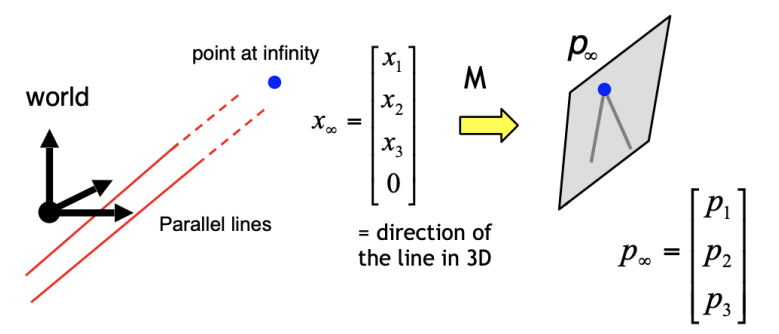
\includegraphics[scale=0.65]{figures/vanishingpoints.png}
	\caption{Vanishing points在world coordinate中的示意图}
	\label{}
\end{figure}

\begin{wrapfigure}{r}{4cm}
	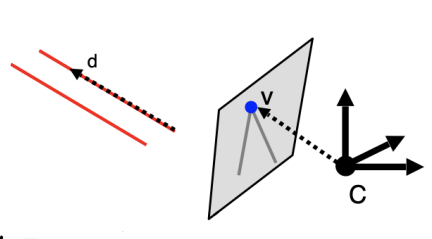
\includegraphics[scale=0.5]{figures/vpanddir.png}
	\caption{相机坐标下的方向}
\end{wrapfigure}
上图的坐标是world coordinate当中.如果是在camera coordinate当中,设$\bm d = (a, b, c)$是直线的方向向量,$\bm v$代表消失点,我们还可以导出如下关系\footnote{注意在右图里,$\bm v$并不是从相机坐标中心出发的三维矢量,而是图片坐标下的齐次坐标.}:
\begin{equation}
	\bm v = \bd K \bm d
\end{equation}


这一点不难证明:由于是在相机坐标之下,无需考虑extrinsic参数,直接有
\begin{equation}
	\bm v = \bd M \bm x_\infty = \bd K 
	\begin{bmatrix}
		\bd I & \bm 0
	\end{bmatrix}
	\begin{bmatrix}
		a\\b\\c\\0
	\end{bmatrix} = \bd K \bm d
\end{equation}

这样,如果已知vanishing point的坐标和相机参数,我们可以知道相机坐标下的这一组平行线的方向:
\begin{equation}
	\bm d = \frac{\bd K^{-1} \bm v}{\norm{\bd K^{-1} \bm v}}
\end{equation}






\begin{wrapfigure}{r}{4cm}
	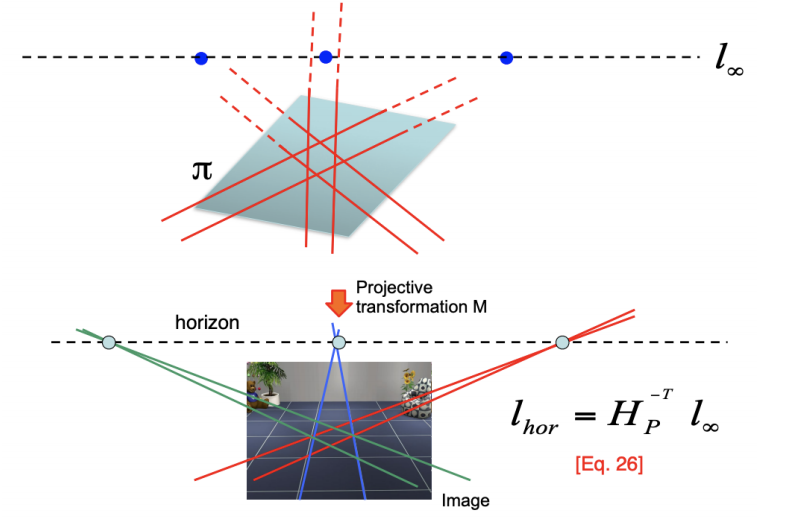
\includegraphics[scale=0.35]{figures/horizon.png}
	\caption{天际线}
\end{wrapfigure}

如果我们继续推广在二维空间中的结论,那么一系列平行平面将会相交于无穷远处的一条线$l_\infty$.将这条线也作同样的变换,就可以得到Vanishing Line,即Horizon,译为天际线,也就是3维空间$l_\infty$在二维的投影:
\begin{equation}
	l_{\text{hor}} = \bd H^{-\top} l_{\infty}
\end{equation}


通过这种方式,我们可以确定两条线是否平行.首先找出天际线,如果照片上的两条线交于天际线的同一点则平行,反之不平行.

我们还可以通过两个vanishing point确定其对应的平行线之间的夹角.

\begin{wrapfigure}{r}{4cm}
	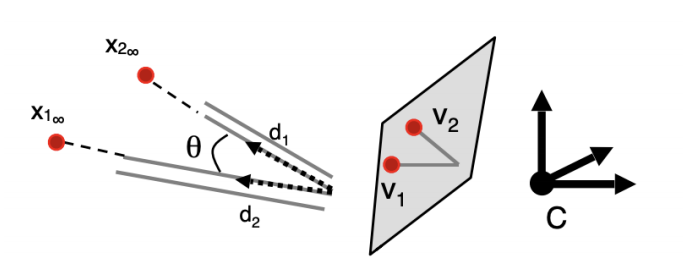
\includegraphics[scale=0.4]{figures/angle_between_line.png}
	\caption{Angle from two vanishing points.}
\end{wrapfigure}

如右图,根据$\bm d = \bd K^{-1} \bm v$,我们可以求出其夹角:
\begin{equation}
	\cos \theta = \frac{\bm d_1 \cdot \bm d_2}{\norm{\bm d_1} \norm{\bm d_2}}
\end{equation}



令$\bm \Omega =\left(K K^{T}\right)^{-1}$,得到
\begin{equation}
	\cos \theta=\frac{\bm{v}_{1}^{\top} \bm \Omega \bm{v}_{2}}{\sqrt{\bm{v}_{1}^{\top} \bm \Omega \bm{v}_{1}} \sqrt{\bm{v}_{2}^{\top} \bm \Omega \bm{v}_{2}}}  
\end{equation}

当$\theta = \frac{\pi}{2}$的时候有$\bm{v}_{1}^{\top} \bm \Omega \bm{v}_{2} = 0$.$\bm \Omega$有五个独立变量.如果我们已知空间中的三组互相垂直的平行线和它们在图片上的vanishing point,则我们可以获得三个方程
\begin{equation}
	\begin{cases}
		\bm{v}_{1}^{\top} \bm \Omega \bm{v}_{2} = 0
		\\
		\bm{v}_{1}^{\top} \bm \Omega \bm{v}_{3} = 0
		\\
		\bm{v}_{2}^{\top} \bm \Omega \bm{v}_{3} = 0
	\end{cases}
\end{equation}

如果我们假定相机具有零偏置和方形像素,那么不难得到
\begin{equation}
	\bd K = 
	\begin{bmatrix}
		\alpha & 0 & c_x
		\\ 
		0 & \alpha & c_y
		\\
		0 & 0 & 1
	\end{bmatrix}, \quad
	\bd K \bd K^{\top} = 
	\begin{bmatrix}
		\alpha^2 + c_x^2 & c_x c_y & c_x
		\\
		c_x c_y & \alpha^2 + c_y^2 & c_y
		\\
		c_x & c_y & 1
	\end{bmatrix}
\end{equation}
\begin{equation}
	\bd \Omega = \xk{\bd K \bd K^{\top}}^{-1} = \frac{1}{\alpha^4}
	\begin{bmatrix}
		\alpha^2 & 0 & -\alpha^2 c_x
		\\
		0 & \alpha^2 & -\alpha^2 c_y
		\\
		-\alpha^2 c_x & -\alpha^2 c_y & (\alpha^2 + c_x^2)(\alpha^2 + c_y^2) - c_x^2 c_y^2
	\end{bmatrix}
\end{equation}

$\bm \Omega$的形式变为:
\begin{equation}
	\bm \Omega = 
	\begin{bmatrix}
		\omega_1 & 0 & \omega_4
		\\
		0 & \omega_1 & \omega_5
		\\
		\omega_4 & \omega_5 & \omega_6
	\end{bmatrix}
\end{equation}

四个变量,三个线性方程,在常数倍意义下我们可以得到$\bd \Omega$,随后运用Cholesky分解得到$\bd K$.之后我们就可以对场景进行三维重建,例如计算图片中所有平面的方向,因此一张图片实际上蕴含了周围场景的丰富信息.

在这一节的最后,我们仍然要指出,单纯从一张图片是不可能完整重建原3D场景的,这是因为物体的深度和大小之间存在ambiguity.在下一节当中,我们会试图解决这个问题.